
\section*{7.4 Sine models} 

\subsection*{Exercises}

\begin{enumerate}

\item %workbook 1
Sara and her brother Nahiz run a small coffee shop, Qamaria Cafe.  The basement serves as storage and tends to be fairly humid so they run a dehumidifier to remove water from the air. The dehumidifier automatically cycles on and off.  When it turns off, the humidity rises a bit and when it turns back on, the humidity falls again.  The humidity ($H$\%) depends on the time ($T$ hours) where we measure time from 12:00 PM (midnight) when the machine turns off.  An equation describing this dependence is 
$$H = 10\sin(90T)+45$$
where the sine function is set to take inputs in degrees.
\begin{enumerate}
    \item According to the equation, what is the humidity level at midnight? Hint: $T=0$. \vfill
    \item Make a table showing the humidity at midnight, 1:00 AM, 2:00 AM, 3:00 AM, 4:00 AM, 5:00 AM, 6:00 AM, 7:00 AM and 8:00 AM. \vfill \vfill \vfill
    
    \newpage %%%%%
    
    \item Draw a graph illustrating the relationship.
    
    \bigskip    
    \begin{center}
\scalebox {.8} {\includegraphics [width = 6in] {Graphics/GraphPaper.jpg}}
\end{center}
\bigskip
     
    \item What is the average humidity level? Hint: it's the height of the midline of the graph. \vfill 
    \item How often does the humidifier make a full cycle (on/off)?  Hint: it's the period. \vfill
\end{enumerate}

\vfill \vfill \vfill

\newpage %%%%%

\item %workbook 2

Sara's specialty is lattes -- hot espresso coffee with steamed milk. Qamaria Cafe's monthly latte revenue goes up and down depending on the season.  Based on data from 2025, Sara estimates that 
$$R=6000\sin(30M)+8000$$
where
$$M = \text{ time (in months since October 2025) } \sim \text{ indep}$$
$$R = \text{ latte revenue (in \$) } \sim \text{ dep}$$
and the sine function is set to take inputs in degrees.

Nahiz drew a graph showing three years of expected revenue if Sara's model continues.

\begin{center}
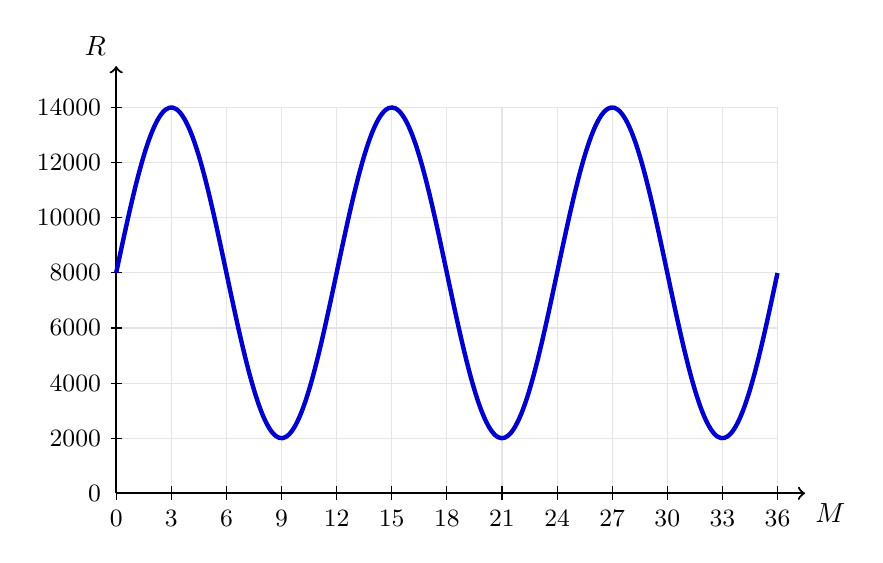
\begin{tikzpicture}[xscale=0.2333, yscale=0.35]
    % Grid lines (horizontal)
    \draw[gray!20, line width=0.4pt] (0,2) -- (36,2);
    \draw[gray!20, line width=0.4pt] (0,4) -- (36,4);
    \draw[gray!20, line width=0.4pt] (0,6) -- (36,6);
    \draw[gray!20, line width=0.4pt] (0,8) -- (36,8);
    \draw[gray!20, line width=0.4pt] (0,10) -- (36,10);
    \draw[gray!20, line width=0.4pt] (0,12) -- (36,12);
    \draw[gray!20, line width=0.4pt] (0,14) -- (36,14);

    % Grid lines (vertical)
    \foreach \x in {0, 3, 6, 9, 12, 15, 18, 21, 24, 27, 30, 33, 36} {
        \draw[gray!20, line width=0.4pt] (\x,0) -- (\x,14);
    }

    % Axes
    \draw[->, thick] (0,0) -- (37.5,0) node[below right] {$M$};
    \draw[->, thick] (0,0) -- (0,15.5) node[above left] {$R$};

    % Y-axis ticks and labels
    \foreach \y/\label in {2/2000, 4/4000, 6/6000, 8/8000, 10/10000, 12/12000, 14/14000} {
        \draw (0.3,\y) -- (-0.3,\y) node[left] {\small\label};
    }
    \node[left] at (-0.3,0) {\small 0};

    % X-axis ticks and labels (3 years / 36 months)
    \foreach \x in {0, 3, 6, 9, 12, 15, 18, 21, 24, 27, 30, 33, 36} {
        \draw (\x, 0.25) -- (\x, -0.25) node[below] {\small\x};
    }

    % Plot the Sine Curve R = 6*sin(30*M) + 8
    \draw[smooth, ultra thick, blue!80!black, domain=0:36, samples=200] 
        plot (\x, {6*sin(30*\x) + 8});
\end{tikzpicture}
\end{center}

\begin{enumerate}
    \item According to the equation, what is the latte revenue in October 2026?  Indicate the point on the graph that shows the answer. \vfill
    \item According to the graph, what is the highest latte revenue and in which month of the year does it occur? Explain why your answer makes sense. \vfill
    
    \newpage %%%%%
    
    \item According to the graph, what is the lowest latte revenue and in which month does it occur? Explain why your answer makes sense.  \vfill
    \item According to the graph, what is the period of this sine model and what does it mean in the story?  \vfill
    \item How could we calculate the period of this sine model from the equation? \vfill
    \item If we were to include iced latte sales, how do you think the graph would change?  Note: iced latte's are lovely when it's hot out! \vfill
\end{enumerate}

\newpage %%%%%

\item %workbook 3
Inside a car's engine, controlled micro-explosions of gasoline push a metal cylinder called a piston up and down. The piston's movement turns these explosions into rotational force that powers the vehicle's wheels.  When a car is parked with its engine running (idling) the height, $H$ cm, of the middle of the piston (above the base) is given by the equation
$$H=4 \sin(4500S) + 10$$
where $S$ is the time since the car started, measured in seconds and the sine function is set to take inputs in degrees.

\begin{enumerate}
    \item Make a table showing the height of the middle of the piston after 0, .02, .04, .06, .08, .10, .12, .14, .16, .18, and .20 seconds.  \vfill 
    \item Use the equation to find the period and explain what it means in the story. \vfill
    
    \newpage %%%%%
    
    \item Draw a graph showing the height of the piston for the first .02 seconds.
 
    \begin{center}
\scalebox {.8} {\includegraphics [width = 6in] {Graphics/GraphPaper.jpg}}
\end{center}
\bigskip

    \item What does the constant 10 mean in the story and what are its units? \vfill
    \item What does the 4 mean in the story and what are its units? \vfill
    \item Indicate where we can see 10, 4, and .08 on the graph. \bigskip
    \item The car's engine runs at .08 seconds per cycle.  Convert units to see that the car's engine runs at 12.5 cycles per second. \vfill \vfill
    \item Convert units to calculate the RPM, which is revolutions (or cycles) per minute. \vfill \vfill
\end{enumerate}

\newpage %%%%%

\item %workbook 4
Ocean tides force seawater to flow back and forth through a narrow opening into a bay. At midnight on Monday, the water reached ``slack tide'', momentarily stopping before it began flowing inward. The water's speed (measured in knots) changes continuously: positive values mean water is rushing into the bay, while negative values mean water is flowing out toward the ocean. The water reaches a maximum inward speed of $+4\text{ knots}$, drops back to $0\text{ knots}$ at slack tide, reaches a peak outward speed of $-4\text{ knots}$, and then returns to $0\text{ knots}$ to repeat the process. This complete back-and-forth cycle repeats every 12 hours and 25 minutes. 

This water flow can be modeled with a sine equation where 
$$H = \text{time (hours since midnight)} \sim \text{indep}$$
$$S = \text{water's speed (knots)} \sim \text{dep}$$
and the sine function is set to take inputs in degrees.

\begin{enumerate}
    \item According to the story, what is the midline of the sine model?  Hint: it occurs at the slack tide. \vfill
    \item According to the story, what is the amplitude of the sine model? \vfill
    \item According to the story, what is the period of the sine model? \vfill
    \item Convert 12 hours and 25 minutes to decimal hours. \vfill
    \item Write an equation showing how the water's speed varies over time.  Hint: You will need to use the number 360 and your answer to (d) to find the constant multiplying $H$ in the equation. \vfill \vfill \vfill
\end{enumerate}

\end{enumerate}

